\section{Customer Perspectives}
\label{sec:customer_perspective}

In order to develop a successful business model, it is crucial to first understand the customer's
perspective. This customer-centricity allows to develop a business innovation and business model
that is tailored to the customer's needs and drivers, thereby increasing the chances of success.
In particular, the innovation solution should be challenged at any stage of the development process.
In this section, we will thus first identify the different customer segments in career counseling,
and then further elaborate a persona for one of the customer segments. A persona is a fictional
character that represents a customer segment and their specific needs and drivers.

Career counseling can be provided to a wide range of different clients. Especially, clients may be
in different stages of their career. A client may be in the process of finishing school or university
and about to enter the job market. Another client might already have several years of work experience
and looking to optimize his or her career. A third client may be in the process of re-entering the job
market after a period of absence, such as unemployment or a parental leave. Due to these totally different
\textit{life circumstances}, the customer perspectives might be entirely different. Considering the
Maslow pyramid of needs \citep{maslowTheoryHumanMotivation1943}, a client in the process of re-entering
the job market might be more concerned with the basic needs (such securing access to food and shelter)
than a client who has an established career and is seeking a career optimization. The latter might be
more concerned with the higher needs of self-actualization. Although we will subsequently only develop
a persona for one customer segment, we nevertheless want to shed light on the individual needs of these
three client archetypes.

\subsection{Job Market Entry}

Graduates and other job market entrants are often faced with the challenge of finding a suitable job. As
they do not have previous work experience (or just a little), they face challenges in finding a job that
matches with their education, skills and interests. They often lack the necessary knowledge to successfully
apply for a job. Job market entrants may also lack knowledge about the employer or its industry potentially
leading to a mismatch between the entrant's expectations and the reality of the job.
\newline

\noindent\textbf{Needs:}

\begin{itemize}
    \item \textit{personalized} advice and coaching
    \item covering basic needs by generating sufficient income from employment
    \item information on the job market
    \item information on the application process
    \item assessment of skills, interests and cultural \& ethical values
    \item job recommendations matching with education, skills, interests and cultural \& ethical values
    \item assistance in preparing the CV and writing a cover letter
    \item coaching for job interviews
\end{itemize}

\newpage
\subsection{Career Transition}

Professionals with a few years of work experience may be looking to optimize or change their career by either 
transitioning into a new role with more responsibility, by changing into another industry, or by choosing a new
career path. They may be looking for a new role in order to grow and advance their career. Others may be unsatisfied
with their current job, career advancement prospects, or industry and hence looking to change their career path entirely. 
This customer segment is different from the job market entrants, as they have already gained some work experience and
have a better understanding of their skills, interests and values. Further, the focus is on psychological safety and
self-actualization, as the basic needs are already met. However, transitioning to a new role or new career path may
also pose significant risks. The career move may turn out differently than expected, and the new role or career path
may not be a good fit. This may lead to a loss of self-esteem, confidence and motivation. In the worst case, this could
translate to lower job performance, a loss of the job and hence of income.
\newline

\noindent\textbf{Needs:}
\begin{itemize}
    \item \textit{personalized} advice and coaching
    \item high safety in the career transition, e.g., by choosing industry and career path transitions that are common
        and typically successful
    \item development of a personal career plan
    \item assessment of skills gaps and development of a plan to close these gaps
    \item assistance in job search, e.g., by providing matching job recommendations
    \item coaching relative to the new industry and role
\end{itemize}
\vspace*{0.1cm} 

\subsection{Seeking Reintegration into the Job Market}

Clients who are seeking reintegration into the job market may have been unemployed for various reasons and over
different periods of time. They may have been unemployed for a short time, e.g., after a parental leave, or for
a longer time, e.g., due to a layoff in an economic downturn. Also, they may have been working in a different
country previously and following their spouse to a new country as part of an expatriation or international
relocation. Whatever the reason and length of absence from the job market, this customer segment shares a
common overarching need: they are looking to re-enter the job market and find a suitable job as quickly as
possible---the longer the absence from the job market, the more difficult it gets to re-enter.

\subsection{Developing a Persona}

In the following we elaborate the persona of Sarah, a recent graduate who is about to enter the job market. We will
describe her background, goals, and needs in order to better understand her current perspective on career counseling.
We will also think about how Sarah might use career counseling during the first few years of her career, i.e., as
a \textit{young professional}.
\newline

\noindent \textbf{Name:} Sarah
\newline\noindent\textbf{Age:} 24
\newline\noindent\textbf{Occupation:} Completed graduate studies, about to enter the job market
\newline\noindent\textbf{Education:} Tertiary
\newline\noindent\textbf{Income:} Lower middle class

\noindent\textbf{Background:} Sarah is a recent graduate who is feeling a mix of emotions as she prepares to enter the job market.
She is excited about the opportunities that lie ahead but also nervous about the challenges she may face during this transition in
her life. She values her cultural and ethical beliefs and seeks to find an employer and industry that align with those values. Sarah
wants her career to be a reflection of her principles and make a positive impact in the world, while also providing opportunities for
personal and professional growth.

\begin{figure}[h!]
    \centering
    \caption{Persona of Sarah}
    \label{fig:persona}
    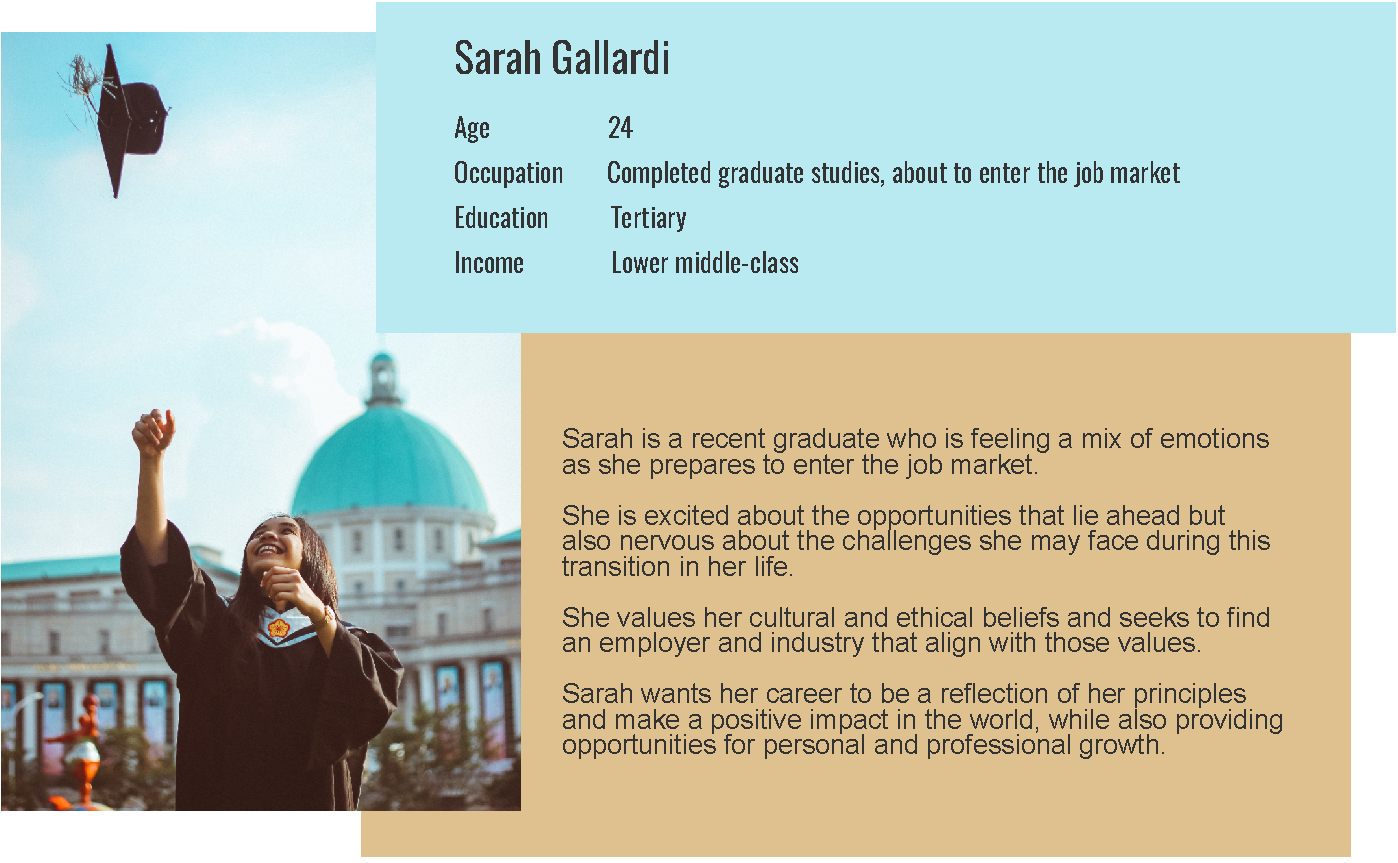
\includegraphics[width=\linewidth]{persona.pdf}
\end{figure}

\noindent\textbf{Goals and Needs:}

\begin{itemize}
    \item \textbf{Cultural and Ethical Alignment:} Sarah places a high value on cultural and ethical alignment with potential employers and certain industries. She seeks organizations that promote diversity, inclusion, and equality. She wants to work in an environment that respects and values different perspectives and cultures.
    \item \textbf{Sustainable Practices:} Sarah is passionate about sustainability and environmental responsibility. She is keen on working in industries that prioritize sustainable practices, such as renewable energy, green technologies, or eco-friendly initiatives. She wants to contribute to a better future through her career choices.
    \item \textbf{Social Impact:} Sarah wants her work to have a positive impact on society. She seeks opportunities in industries such as nonprofit organizations, social enterprises, or companies with a strong corporate social responsibility focus. She wants to make a difference and improve the lives of others through her career.
    \item \textbf{Ethical Business Conduct:} Sarah believes in conducting business ethically and responsibly. She values organizations that prioritize transparency, integrity, and ethical decision-making. She wants to work for employers who uphold high ethical standards and prioritize the well-being of employees and stakeholders.
    \item \textbf{Cultural Diversity and Inclusion:} Sarah values workplaces that foster cultural diversity and inclusion. She seeks employers who celebrate and embrace individuals from different backgrounds, perspectives, and experiences. She wants to work in an environment that promotes equality and offers equal opportunities for career growth.
    \item \textbf{Work-Life Balance:} Sarah recognizes the importance of work-life balance in maintaining her well-being and overall satisfaction. She prefers employers and industries that prioritize a healthy work-life balance, offer flexible working arrangements, and support employee well-being initiatives.
    \item \textbf{Learning and Development:} Sarah seeks employers and industries that prioritize continuous learning and development. She values organizations that provide opportunities for professional growth, training programs, mentorship, and support for employees' career advancement.
\end{itemize}

\noindent\textbf{Summary:}
Overall, Sarah wants to find an employer and industry that not only align with her cultural and ethical values but also provide
opportunities for personal and professional growth. She aspires to contribute to a sustainable, socially responsible, and inclusive
work environment where she can make a positive impact and thrive in her career.
Considering Maslow's hierarchy of needs, Sarah is currently in the process of fulfilling her basic needs by seeking an employment
that will secure food, shelter, etc. However, she also has highers aspirations: she strives to fulfill her psychological needs, such as
belongingness and esteem. The right job with the right employer will provide her with a sense of belonging and self-esteem. She wants to
feel valued and appreciated for her contributions, while being able to her career. Finally, aligning her cultural and ethical values with
her career choices will allow her to partly fulfill her self-actualization needs.
